% #############################################################################
% This is Chapter 8
% !TEX root = ../main.tex
% #############################################################################
\fancychapter{Fault Injection}
\label{chap8:fatori_fi}



% -------------------------------------------------------------
\section{System Overview}
\label{chap8:fi_workflow}

The \ac{FI} system developed for this work is implemented as standalone \ac{FI} tool, invoked by \ac{Fatori-V} when \ac{FI} is enabled. The tool defines each campaign by combining temporal and spatial distributions, called Area and Time Profiles. The tool supports both configuration memory and \ac{FF}/register injections: configuration memory injections are executed through \ac{SEM}, while register injections require a dedicated on-chip hardware path because \ac{SEM} only targets configuration memory. The selected Area Profile builds the injection target pool, and the Time Profile schedules the injections.

The main entry file is \texttt{fault\_injection.py}, which executes the flow shown in \Cref{fig:fi_flow}. The tool starts by parsing the \ac{CLI} and loading the System Dictionary, which describes the board, pblock bounds, and register IDs. It then initializes logging and sets the campaign seeds.

\begin{figure}[h]
  \centering
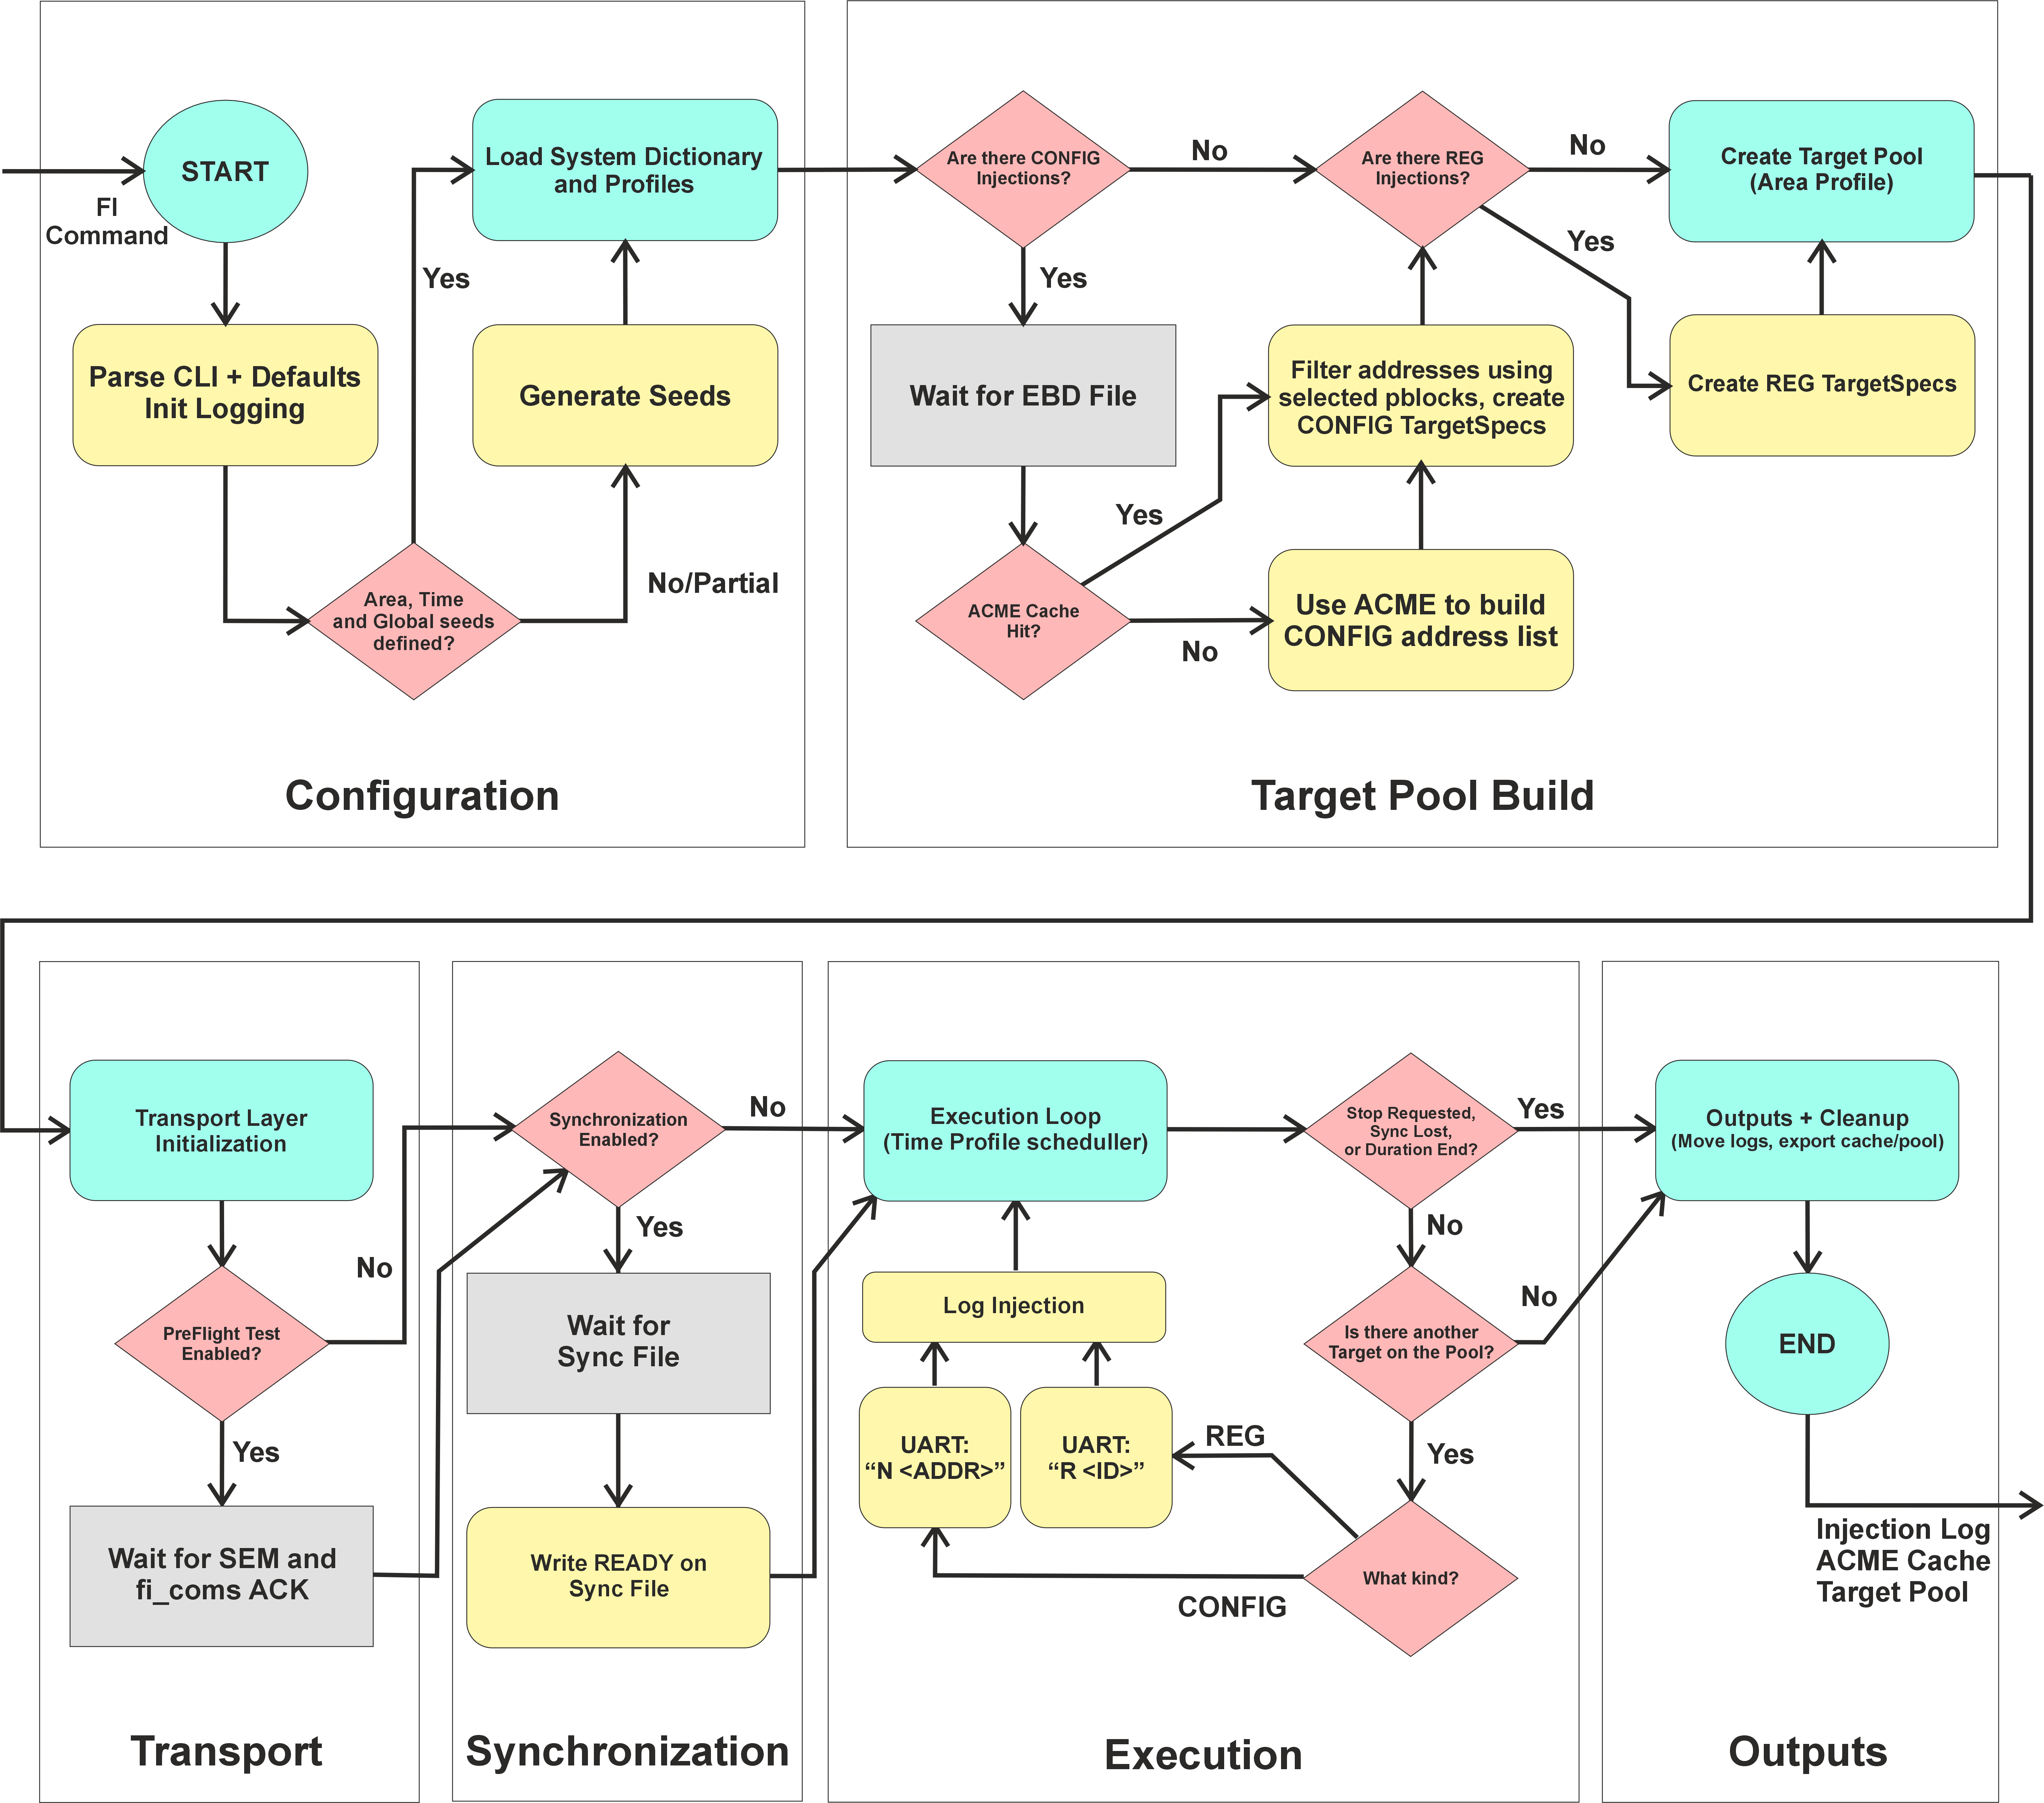
\includegraphics[width=0.8\linewidth]{Images/chap8_fi_system.png}
  \caption{Fault Injection flow phases.}
  \label{fig:fi_flow}
\end{figure}

The selected Area Profile builds an ordered list of injection targets. Register targets store the register identifier used by the hardware injection path. Configuration memory targets store addresses generated with \ac{ACME}, which maps selected pblock regions into \ac{EBD} entries and converts them into \ac{SEM} injection addresses. Previously generated \ac{ACME} results can be loaded from cache when the same pblock and \ac{EBD} pair is reused.

After the target list is built, the respective transport layer is activated. If synchronization is enabled, the tool waits for the benchmark start signal before injecting. 

During execution, the Time Profile fetches injections from the built pool, waits according to its schedule, and routes each target to the correct injection path. Both paths share the external \ac{FI} \ac{UART} connection to the \ac{FPGA}, but use different command formats. Configuration memory targets are sent to \ac{SEM}. Register targets have their identifier broadcasted to the pipeline. 

The campaign ends when the timing policy finishes, the target pool is exhausted, synchronization is lost, or an external stop is requested. The tool outputs the injection log, the generated target list, and the \ac{ACME} cache files to the output path provided through \ac{CLI}.



% -----------------------------------
\subsection{Injection Targets}
\label{chap8:fi_targets_specs}

The \ac{FI} tool represents each injection as one target record, which stores the information needed to execute the injection independently of its type. Area Profiles merge multiple target records to build an ordered target pool. Time Profiles can schedule injections from that pool. A reduced example of a target pool is shown in \Cref{lst:tpool_example}.


\begin{lstlisting}[float=h,caption={Reduced example of a mixed target pool.},label={lst:tpool_example}]
targets:
  - kind: CONFIG
    module_name: "alu"
    config_address: "00001234"
    pblock_name: "alu_pb"
    source: "profile:modules"

  - kind: REG
    module_name: "ibex_id_stage"
    reg_id: 93
    reg_name: "imd_val_q_reg_0"
    source: "profile:modules"
\end{lstlisting}


\texttt{CONFIG} targets represent configuration memory injections executed through \ac{SEM}. They store the \ac{SEM} address and the pblock name used in logs. \texttt{REG} targets represent register injections executed through the hardware path described in \Cref{chap8:fi_reg_injections}. They store the 8-bit register identifier and the register name used in logs.

The generated pool can be exported to a \texttt{.yaml} file, so that later campaigns can reload that file through the \texttt{target\_list} Area Profile. This allows a campaign to be repeated without running target expansion again, and improves reproducibility. 







% -------------------------------------------------------------
\subsection{User Interface and System Inputs}
\label{chap8:fi_user_interface}

The \ac{FI} tool is configured through the \ac{CLI}. The command selects the board, serial port, baud rate, seeds, System Dictionary, \ac{EBD} file, Area Profile, Time Profile, and profile-specific arguments. A reduced example is shown in \Cref{lst:fi_cli_example}.

\begin{lstlisting}[float=h,caption={Reduced example of the FI CLI usage.},label={lst:fi_cli_example}]
python3 -m fi.fault_injection
  --board xcku040 --dev /dev/ttyUSB0 --baud 115200
  --global-seed 123 --log-level normal
  --system-dict system_dict.yaml
  --ebd build_v1.ebd 
  --area modules --area-args targets=ibex_alu,ratio=1,target_mode=sequential 
  --time poisson --time-args rate_hz=5,duration_s=60

\end{lstlisting}

The System Dictionary \texttt{.yaml} file is always required. It defines the target board, the pblock bounds of each injectable module, and the register IDs associated with each module. The \ac{EBD} file is required only when configuration memory injections are enabled, because \ac{ACME} uses it to map pblock regions into \ac{SEM} injection addresses.

For standalone use, the user must provide a System Dictionary that describes the current architecture. In \ac{Fatori-V}, the System Dictionary is generated by the Pblock Sizing Model described in \Cref{chap7:pblock}. An example System Dictionary is provided in \Cref{app_c:system_dict}.

Other inputs depend on the selected profiles. An Area Profile can load a user-provided \texttt{TargetPool} \texttt{.yaml} file instead of generating one, as described in \Cref{chap8:fi_area}. A Time Profile can also require an external trace file, as described in \Cref{chap8:fi_time}. The \ac{EBD} file is generated in Vivado by setting the \texttt{BITSTREAM.SEU.ESSENTIALBITS} property before bitstream generation.






% #############################################################################
\section{Fault Injection Software}
\label{chap8:fi_software}

This section details how the Area and Time Profiles used to build and schedule the injections were implemented.

% -------------------------------------------------------------
\subsection{Spatial Fault Distributions}
\label{chap8:fi_area}

Spatial fault distributions are implemented as Area Profiles and convert a requested injection scope into an ordered target pool. The pool may contain \texttt{CONFIG} targets, \texttt{REG} targets, or both. When both are enabled, the user can define the intended share of \texttt{REG} targets.


Each Area Profile follows the fixed interface shown in \Cref{app_e:area_prof}. It receives the System Dictionary, the board name, the \ac{EBD} path, and profile-specific arguments. If a required argument is missing and has no default, the \ac{FI} tool reports an error. This interface allows users to add new spatial distributions, keeping the \ac{FI} tool modular.

The native Area Profiles are \texttt{device}, \texttt{modules}, and \texttt{target\_list}. The \texttt{device} profile builds targets across the full device. Configuration memory targets are generated from the full-device bounds through \ac{ACME}, while register targets are taken from the board register list in the System Dictionary. The user can select whether targets are kept in order or shuffled, set the share of register targets, and enable target repetition up to a configured pool size.

The \texttt{modules} profile restricts injections to selected hardware modules. For each selected module, the profile derives configuration memory targets from its pblock bounds and register targets from its register list. The user can specify which modules to include or exclude, how modules are selected during pool construction (randomly, round-robin, or sequentially), and whether targets within each module are kept in order or shuffled.

The \texttt{target\_list} profile loads an existing target pool from a \texttt{.yaml} file. This profile does not use the System Dictionary, board name, or \ac{EBD} path, because the target list is already defined. It is used to replay a previous campaign or to run a manually defined target sequence.





% -------------------------------------------------------------
\subsection{Mapping Essential Bits to Injection Addresses}
\label{chap8:fi_acme_impl}

This subsection describes how the \ac{FI} tool converts a given pblock into injection addresses for the \ac{SEM} for \texttt{CONFIG} targets, implementing the \ac{ACME} equations introduced in \Cref{chap8:fi_sem_theory,chap8:fi_acme_theory}. 

The \ac{ACME} inputs are the pblock bounds, the \ac{EBD} file generated by Vivado, and the board-specific mapping constants. \ac{ACME} uses the pblock bounds to select the relevant \ac{EBD} entries, then converts each selected essential bit into the \(\{LA,WD,BT\}\) tuple required by \ac{SEM}. The output is a list of \ac{SEM}-ready addresses used by the Area Profile when building \texttt{CONFIG} targets.

The mapping uses three representations of the same bit. The target pblock is described in Vivado tile coordinates \((X,Y)\). The \ac{EBD} file stores each essential bit as a payload-line position \((L,p)\), where \(L\) is the payload line index after the header and \(p\) is the position of a \texttt{1} inside that line. \ac{SEM} receives the injection address as \(\{LA,WD,BT\}\), where \(LA\) is the linear frame address, \(WD\) is the word index inside the frame, and \(BT\) is the bit index inside the 32-bit word.

The \ac{FI} tool applies \ac{ACME} in two steps. First, it expands the \ac{EBD} file by converting each \ac{EBD} bit \((L,p)\) into a \(\{LA,WD,BT\}\) tuple using \Cref{eq:acme_ebd_to_lawdbt}. Then, it filters the expanded tuples, keeping only the ones whose estimated physical position belongs to the requested pblock. This second step is board-dependent.

For Basys3, each expanded tuple is assigned to a horizontal band using \Cref{eq:basys3_band_from_la}. The \(X\) coordinate is estimated with \Cref{eq:basys3_x_from_la}, and \(Y\) is assigned as the midpoint of the selected band. The candidate is kept only if the resulting \((X,Y)\) lies inside the pblock rectangle.

\begin{equation}
  band = \left\lfloor \frac{LA}{FY} \right\rfloor
  \label{eq:basys3_band_from_la}
\end{equation}

\begin{equation}
  X \approx X_{\min} + \left\lfloor \frac{(LA \bmod FY)\cdot (X_{\max}-X_{\min})}{FY} \right\rfloor
  \label{eq:basys3_x_from_la}
\end{equation}

For XCKU040, the tool uses a row-dependent linear relation between tile columns and linear frame addresses, shown in \Cref{eq:xcku40_la_from_x}. During filtering, \Cref{eq:xcku40_x_from_la} estimates the tile column from the candidate \(LA\). The \(Y\) coordinate is assigned as the row midpoint, and the candidate is kept only if the estimated point lies inside the pblock rectangle.

\begin{equation}
LA \approx F_X\cdot (X-\texttt{OFFSET\_X}) + \texttt{OFFSET\_Y}(r)
\label{eq:xcku40_la_from_x}
\end{equation}

\begin{equation}
X \approx \texttt{OFFSET\_X} + \left\lfloor \frac{LA-\texttt{OFFSET\_Y}(r)}{F_X} \right\rfloor
\label{eq:xcku40_x_from_la}
\end{equation}

The constants used by both implementations are summarized in \Cref{tab:chap8_acme_constants}.

\begin{table}[h]
\centering
\small
\setlength{\tabcolsep}{3pt}
\renewcommand{\arraystretch}{1.2}
\begin{tabularx}{\textwidth}{|l|X|c|c|X|X|}
\hline
\rowcolor{tableheader}\textbf{Board} & \textbf{Device} & \textbf{\(W_f\)} & \textbf{\(N_\text{dummy}\)} & \textbf{Physical limits and rows} & \textbf{Mapping constants} \\
\hline
\hline
Basys3 & Artix-7 XC7A35T & 101 & 109 & \(X=[0,209]\), \(Y=[0,159]\). Row cut-lines at \(Y=26,53,79,106,132\). & \(FY=3520\), \(FX=22\). \\
\hline
XCKU040 & Kintex UltraScale XCKU040 & 123 & 141 & \(X=[50,357]\), \(Y=[0,309]\). Row cut-lines at \(Y=61,123,185,247\). & \(F_X=17\), \(\texttt{OFFSET\_X}=50\), \(\texttt{OFFSET\_Y}(r)\in\{0,10472,20944,31416,41888\}\). \\
\hline
\end{tabularx}
\caption{Constants used by the \ac{ACME} implementations in the \ac{FI} tool.}
\label{tab:chap8_acme_constants}
\end{table}

The Basys3 and XCKU040 constants were obtained from board documentation when available and from empirical placement experiments in Vivado. Each experiment placed a reference module in known pblocks, generated an \ac{EBD} file, expanded it into \(\{LA,WD,BT\}\) tuples, and fitted the relation between address ranges and physical coordinates.





% #############################################################################
\subsection{Temporal Fault Distributions}
\label{chap8:fi_time}

Temporal fault distributions are implemented as Time Profiles and define when injections occur. A Time Profile consumes the target pool produced by the Area Profile, requests one target at a time, waits according to its scheduling rule, and sends the target to the correct backend.

Each Time Profile follows the fixed interface shown in \Cref{app_d:time_prof}. It receives profile-specific arguments, the selected seed, and the global settings. If a required argument is missing and has no default, the \ac{FI} tool reports an error. This interface allows users to add new temporal distributions, keeping the \ac{FI} tool modular. All profiles accept an optional campaign duration limit.

The native Time Profiles are \texttt{uniform}, \texttt{ramp}, \texttt{poisson}, \texttt{microburst}, \texttt{mmpp2}, and \texttt{trace}. The \texttt{uniform} profile injects at a constant rate, defined either as a fixed period or as a frequency.

The \texttt{ramp} profile changes the injection rate linearly between a start and end rate over a configured duration. The implementation updates the rate after each injection, computes the next period from the current elapsed time, and advances the next deadline accordingly.

The \texttt{poisson} profile samples exponential inter-arrival times at a configured average rate. The implementation uses a local \ac{RNG} to sample each delay, and stops when the next sampled injection would exceed the campaign duration.

The \texttt{microburst} profile alternates burst and idle intervals, each with a configurable rate and duration. If the idle rate is set to zero, the idle interval contains no injections.

The \texttt{mmpp2} profile implements a two-state Markov-modulated Poisson process. The user configures the low and high injection rates, the transition probabilities between states, and optionally the initial state and seed. The implementation samples the next Poisson delay from the current state rate and applies the transition probabilities after each injection.

The \texttt{trace} profile replays injection times from a user-provided text file. The user selects whether the file values are absolute timestamps or relative gaps, and can configure the number of replay passes. The implementation ignores blank lines and comments.










%##########################################################
\section{Implemented Fault Injection Hardware}
\label{chap8:fi_hardware}

The \ac{FI} hardware provides the on-chip support needed to execute the injections schedulled by the \ac{FI} tool. Configuration memory injections are executed by Xilinx's \ac{SEM} \ac{IP}, while register injections use locally developed hardware.




% -----------------------------------
\subsection{Flip-Flop and Register Injections}
\label{chap8:fi_reg_injections}

The register-injection system was created because \ac{SEM} only injects faults in configuration memory. The goal was to support register faults with a scalable mechanism that does not require a dedicated control path for each register. The solution uses one broadcast register ID and one common self-injection wrapper developed in this work.

A register-injection command starts with the \texttt{R} byte and is followed by an 8-bit register ID. These commands go through the \ac{FI} \ac{UART} controller, which decodes them and broadcasts the 8-bit register ID. 

All \ac{FI}-enabled pipeline registers have a fixed local ID and compare it with the listened broadcast value. When both IDs match, only that register stores an injection request. Each register ID is unique and is hardcoded into the module.

When \ac{FI} is enabled, the default register wrapper is replaced by the developed self-injection wrapper. The wrapper keeps the normal register interface and adds the broadcast input described in \Cref{chap8:fi_coms}. Internally, it compares the received broadcast ID with its own fixed ID and stores a match as a pending injection request. This stored request avoids losing the injection when the broadcast lasts only one cycle.

The fault is applied only when the register is not being written. If a write is pending, the injection request is held and the normal write is preserved. When the register becomes idle, the wrapper forces a local write with the stored value XORed with a fixed mask. In the current implementation, the mask flips the middle bit of the stored word. After the flip is applied, the pending request is cleared.




% -----------------------------------
\subsection{Injection \ac{UART} Router}
\label{chap8:fi_coms}

The \ac{FI} hardware uses a developed \ac{UART} router to connect the external \ac{FI} \ac{UART} to the injection paths. The router, the \ac{SEM} \ac{IP}, and the broadcast wiring are gated and are only generated when \ac{FI} is enabled.

The router listens to the \ac{FI} \ac{UART} and intercepts register-injection \texttt{R} commands. When the incoming byte is not \texttt{R}, the command stream is forwarded to \ac{SEM}'s \ac{UART}, preserving the interface described in \Cref{chap8:fi_sem_theory}. When the router receives an \texttt{R} byte, it captures the following byte as the register ID, stores it in an internal FIFO, and later broadcasts it through a dedicated hardware signal for one clock cycle.

The broadcast signal is generated by the injection handler \ac{FSM}. When the FIFO contains an entry, the handler reads the next register ID, drives the signal for one clock cycle, and clears it in the following cycle. This signal is created at the top integration level and propagated through the Ibex hierarchy, connecting to the register wrappers. Each wrapper compares the broadcast ID with its local ID.

The module also exports monitoring pulses for injection counting and latency measurement. One pulse is asserted when a register injection command is accepted, and another when a configuration memory injection command is detected.

The router supports three response modes. In \texttt{Transparent} mode, it provides no debug signals. In \texttt{ACK} mode, it confirms each injection with a single-character response. In \texttt{DEBUG} mode, it reports the register-injection sequence and \ac{SEM} answers for debugging. Normal campaigns disable \texttt{ACK} and \texttt{DEBUG} to reduce \ac{UART} traffic.




% #############################################################################
\section{Additional Features}
\label{chap8:fi_integration}

The \ac{FI} tool includes other support features besides the ones described. This section briefly mentions some.

The \ac{SEM} backend includes an optional preflight check that sends a status command before the campaign starts. This validates the \ac{UART} connection and confirms that \ac{SEM} is responsive before any injection is scheduled.

For high-rate campaigns, \ac{SEM} injections can be sent without waiting for each monitor response. This reduces the influence of \ac{UART} response latency on the Time Profile schedule.

The tool also provides a debug mode, where hardware communication is replaced by stub messages, while target generation, scheduling, logging, and campaign termination remain active.



% #############################################################################
\section{Summary}
\label{chap8:summary}

This chapter presented the fault injection component of the Fatori-V layer. The \ac{FI} system overview was described, covering how Area and Time Profiles define the spatial and temporal distribution of injections across configuration memory and register targets. The \ac{ACME} algorithm was presented as the method for mapping pblock regions to \ac{SEM}-compatible essential-bit addresses, with implementations for the Basys3 and XCKU040 boards. The \ac{FI} hardware was described, including the register injection path and the \ac{UART} router that multiplexes register and configuration memory injection commands. \Cref{chap9:results} presents the experimental results obtained using this infrastructure.

Logging is configurable through verbosity levels and event selection. This allows short logs during normal campaigns and more detailed logs during debugging, without changing the campaign implementation.